

\documentclass[11pt, table, aspectratio=169]{beamer}

%% Note: Beamer is uses' presentation mode' by default (allows for \pause command)
%% adding 'handout' to \document command disables \pause commands
\usepackage[most]{tcolorbox}
\usepackage{xcolor}
\usepackage{listings}
\usepackage{xspace}
\usepackage[export]{adjustbox}
\usepackage{amsmath}
\usepackage{tikz}
\definecolor{codegreen}{rgb}{0,0.6,0}
\definecolor{codegray}{rgb}{0.5,0.5,0.5}
\definecolor{codepurple}{rgb}{0.58,0,0.82}
\definecolor{backcolour}{rgb}{0.95,0.95,0.92}
\usepackage[T1]{fontenc}    % better hyphenation/quotes in monospace
\usepackage[scaled=0.9]{DejaVuSansMono} % optional: nicer monospace font

% Light theme colors
\definecolor{codebg}{RGB}{248,248,248}
\definecolor{codeframe}{RGB}{220,220,220}
\definecolor{javakeyword}{RGB}{0,92,197}
\definecolor{javastring}{RGB}{196,26,22}
\definecolor{javacomment}{RGB}{0,128,0}
\definecolor{javaannotation}{RGB}{170,0,255}
\definecolor{javanumber}{RGB}{120,120,120}

% Optional: handle a few Unicode chars if they appear in code comments
\lstset{
literate={é}{{'{e}}}1 {è}{{`{e}}}1 {à}{{`{a}}}1 {ù}{{`{u}}}1
{É}{{'{E}}}1 {–}{{--}}1 {—}{{---}}1 {“}{{``}}1 {”}{{''}}1
}

%Java style (light)
\lstdefinestyle{javaStyle}{
language=Java,
basicstyle=\ttfamily\small,
keywordstyle=\bfseries\color{javakeyword},
commentstyle=\itshape\color{javacomment},
stringstyle=\color{javastring},
numberstyle=\scriptsize\color{javanumber},
numbers=left,
stepnumber=1,
numbersep=10pt,
backgroundcolor=\color{codebg},
showstringspaces=false,
tabsize=2,
keepspaces=true,
breaklines=true,
frame=single,
rulecolor=\color{codeframe},
captionpos=b,
% Extra Java keywords (modern Java)
morekeywords={var,record,sealed,permits,yield,non-sealed},
% Annotations (common ones)
morekeywords=[2]{@Override,@Deprecated,@SuppressWarnings,@Nullable,@NotNull,@Test},
keywordstyle=[2]\color{javaannotation},
% Emphasise common types
emph={String,Integer,Long,Double,List,Map,Set,Optional},
emphstyle=\color{javakeyword}\bfseries
}

% Dark theme colors
\definecolor{codebgdark}{HTML}{1E1E1E}
\definecolor{codeframedark}{HTML}{3C3C3C}
\definecolor{kwdark}{HTML}{569CD6}
\definecolor{strdark}{HTML}{CE9178}
\definecolor{comdark}{HTML}{6A9955}
\definecolor{annodark}{HTML}{C586C0}
\definecolor{numdark}{HTML}{858585}

\lstdefinestyle{javaDark}{
language=Java,
basicstyle=\ttfamily\small\color{white},
keywordstyle=\bfseries\color{kwdark},
commentstyle=\itshape\color{comdark},
stringstyle=\color{strdark},
numberstyle=\scriptsize\color{numdark},
numbers=left,
stepnumber=1,
numbersep=10pt,
backgroundcolor=\color{codebgdark},
showstringspaces=false,
tabsize=2,
keepspaces=true,
breaklines=true,
frame=single,
rulecolor=\color{codeframedark},
captionpos=b,
morekeywords={var,record,sealed,permits,yield,non-sealed},
morekeywords=[2]{@Override,@Deprecated,@SuppressWarnings,@Nullable,@NotNull,@Test},
keywordstyle=[2]\color{annodark},
emph={String,Integer,Long,Double,List,Map,Set,Optional},
emphstyle=\color{kwdark}\bfseries
}


\newtcolorbox[auto counter,number within=section
]{debox}[1][]{enhanced jigsaw,
colback=green!0!white,
coltext={black},
colframe={black},
coltitle={black},
boxrule=0pt,
frame hidden,
borderline west={1mm}{0mm}{white!50!red},
arc=0mm,
auto outer arc,
boxsep=5pt,
left=4pt,
breakable,
right=4pt,
bottom=0pt,
top=0pt,
before skip=3mm,
after skip=3mm,
%label={def:\thetcbcounter},
#1}

\lstdefinestyle{pythonstyle}{
language=Python,
basicstyle=\ttfamily\small,
keywordstyle=\color{blue},
stringstyle=\color{teal},
commentstyle=\color{gray},
showstringspaces=false,
numbers=none,
frame=single,
breaklines=true,
breakatwhitespace=true,
tabsize=4,
columns=fullflexible
}
\input{LZSCCslides/Header}
\subtitle{LZMSCI521M}
\date{\today}
%\date{}
\author{Dr. Nono S. C. Merleau}
\institute{University of Leipzig/ ScaDS.AI}
\def\week{1}



\newcommand{\gd}[2]{\begin{debox}[label=#1]#2\end{debox}}


\begin{document}

\setcounter{framenumber}{0}
\setcounter{section}{0}

\title{\textbf{Inheritance vs Composition in OOP}}

\maketitle
%


%\begin{frame}{\textbf{What Will You Learn Today?}}
%	%\scriptsize
%	\setbeamertemplate{section in toc}[sections numbered]
%	\tableofcontents[hideallsubsections]
%	%\thispagestyle{empty}
%\end{frame}
%\title{Micro-Course: Inheritance vs Composition in Object-Oriented Programming}
%\author{For First-year Computer Science Students}
%\date{}

\begin{frame}{\textbf{Why Object-Oriented Programming?}}
	
	\begin{enumerate}
		\item We model the world as objects:  \textbf{state} and \textbf{behaviour}.
%		\item OOP helps us build bigger, safer programs by organising code.
%		\item You already use OOP daily: phone apps, games, web backends. 
%	\end{enumerate}
%	\vspace{0.1cm}
%	\textbf{Key Concept}
%	\begin{enumerate}
		\item Class = Mould, a \textbf{blueprint} for object; it defines \textbf{attributes}  and \textbf{methods}.
%		\item Object = Data (\textbf{state}) + Functions (\textbf{behavior}).
		\item Why it matters: \textbf{encapsulation, reuse, polymorphism}.
	\end{enumerate}
	\vspace{0.3cm}
	\textbf{Today you will learn:}
	\begin{enumerate}
		\item Objects vs Classes, state vs behaviours, and examples in \texttt{Java}, \texttt{Python}, and \texttt{UML}.
		\item Relationship between classes: Inheritance vs Composition
	\end{enumerate}
\end{frame}

\section{\textbf{OOP Concepts}}

\begin{frame}[fragile]{\textbf{Notion Of Classes: Basic Syntax}}
	Mould for building Objects: 
	\begin{enumerate}
		\item \textbf{Attributes}: state representation, characteristics
		\item \textbf{Methods}: behaviors, state controller.
	\end{enumerate}
	
	\begin{lstlisting}[style=javaStyle]
public class Rectangle{
	
	Pair<Integer, Integer> p1 = new Pair<Integer, Integer>(1, 2); 
	Pair<Integer, Integer> p2 = new Pair<Integer, Integer>(3, 1); 
	
	// Methods
	public int area() {
		int width = Math.abs(p1.getValue0() - p2.getValue0());
		int height = Math.abs(p1.getValue1() - p2.getValue1());
		return width * height;
	}
}\end{lstlisting}
\end{frame}
%\begin{frame}[fragile]{\textbf{Interfaces and Abstract Classes}}
%\begin{itemize}
%			\item Interfaces are classes that contain methods without implementations
%			\item Abstract classes are classes with at least one method without implementation
%		\end{itemize}
%	\begin{block}{Example}
%\begin{lstlisting}[style=javaStyle]
%public abstract class AbstractRectangle {	
%	Pair<Integer, Integer> p1 = new Pair<Integer, Integer>(1, 2); 
%	Pair<Integer, Integer> p2 = new Pair<Integer, Integer>(3, 1); 
%	
%	//Abstract Methods
%	public abstract int area();
%}\end{lstlisting}
%	\end{block}
%\end{frame}

%\begin{frame}[fragile]{\textbf{Implementating an} \texttt{Interface}}
%	\begin{lstlisting}[style=javaStyle]
%public interface IRectangle {
%	
%	public int area();
%}\end{lstlisting}
%	\begin{lstlisting}[style=javaStyle]
%public class RectangleImpl implements IRectangle {
%	
%	Pair<Integer, Integer> p1 = new Pair<Integer, Integer>(1, 2); 
%	Pair<Integer, Integer> p2 = new Pair<Integer, Integer>(3, 1); 
%	
%	@Override
%	public int area() {
%		// TODO Auto-generated method stub
%		return 0;
%	}	
%}\end{lstlisting}
%
%\end{frame}

\begin{frame}[fragile]{\textbf{Objects}}
%	\begin{block}{What Is An Object?}
		\begin{itemize}
			\item Objects are instances of a class
			\item Objects can also represent different states of a class
			\item Objects are coherent entities that store data and the code (or instructions) working on that data. 
		\end{itemize}
%	\end{block}
	\begin{block}{\textbf{Example}}
\begin{lstlisting}[style=javaStyle]
Rectangle x = new Rectangle()
x.area()\end{lstlisting}

\begin{lstlisting}[style=javaStyle]
Pair<Integer, Integer> p1 = Pair.with(5,2); 
Pair<Integer, Integer> p2 = Pair.with(2, 3);
Rectangle y = new Rectangle(p1, p2);\end{lstlisting}
	\end{block}
\end{frame}

\begin{frame}[fragile]{\textbf{Instantiation (Constructors)}}
	%	When instantiating a class (e.g. \texttt{Rectangle()}), we invoke the\texttt{\_\_init\_\_()} method if it is present in the class's definition.
	\begin{lstlisting}[style=javaStyle]
public class Rectangle{
	Pair<Integer, Integer> p1 = Pair.with(1, 2); 
	Pair<Integer, Integer> p2 = Pair.with(3, 1); 
	
	//Constructor
	public Rectangle(Pair<Integer, Integer>p1, Pair<Integer, Integer> p2) {	
		this.p1= p1; 
		this.p2 = p2; 	 
	}
	// Methods
	public int area() {
		int width = Math.abs(p1.getValue0() - p2.getValue0());
		int height = Math.abs(p1.getValue1() - p2.getValue1());
		return width * height;
	}}\end{lstlisting}
\end{frame}
%\begin{frame}[fragile]{Method and Attributes types: Public, Private, and Protected}
%	
%	\begin{itemize}
	%		\item \textbf{Public}: Visible everywhere (any class, any package), as long as the declaring class itself is accessible.
	%		\vspace{-0.3cm}
	%		\item \textbf{Protected}: Visible to all classes in the same package, and subclasses in any package. 
	%		\vspace{-0.3cm}
	%		\item \textbf{Private}: Visible only within the same top-level class 
	%	\end{itemize}
%	
%	\begin{lstlisting}[style=javaStyle]
	%package oop;
	%		
	%public class Account {
		%	public String owner; 
		%	protected Integer balance; 
		%	private Integer pinCode; // acc.pinCode not allowed out of this class
		%}\end{lstlisting}
%	
%\end{frame}
%\begin{frame}[fragile]{Encapsulation in Python}
%	
%	\textbf{Encapsulation} means:
%	\begin{quote}
	%		Hiding internal data and exposing only a controlled interface.
	%	\end{quote}
%	
%	In Python, encapsulation is achieved by:
%	\begin{itemize}
	%		\item Making attributes \emph{internal} using naming conventions
	%		\vspace{-0.3cm}
	%		\item Accessing data through \emph{public methods}
	%	\end{itemize}
%	
%	\begin{lstlisting}[style=pythonstyle]
	%class Account:
	%	def __init__(self, balance):
	%		self._balance = balance
	%	\end{lstlisting}
%	
%	\begin{itemize}
	%		\item Internal state (\texttt{\_balance}) is hidden
	%		\item Access is controlled via methods
	%		\item Implementation can change without breaking users
	%	\end{itemize}
%	
%\end{frame}

%\begin{frame}[fragile]{Method Chaining}
%	We will see several objects (i.e. Django \texttt{db.models.Model}) that allow for method chaining to construct a pipeline of operations. 
%	
%	We can achieve the same by having our class methods return \texttt{self}.
%	
%	\begin{lstlisting}[style=pythonstyle]
	%class Rectangle:
	%"  "" An abstract representation of a rectangle"""
	%	# Constructor
	%	def __init__(self, p1 = (0,0), p2 = (1,1)):
	%		self.p1 = p1
	%		self.p2 = p2
	%	# Methods
	%	def area(self):
	%		return ((self.p1[0] - self.p2[0])
	%		*(self.p1[1] - self.p2[1]))
	%	\end{lstlisting}
%\end{frame}

%\begin{frame}[fragile]{Methods Overriding: Object String Formatting}
%	
%	All class objects have a default string representation, but it is usually not very useful:
%	
%	\begin{lstlisting}[style=javaStyle]
	%Rectangle rectangle = new Rectangle();
	%System.out.println(rectangle);
	%//oop.Rectangle@5fcfe4b2
	%	\end{lstlisting}
%	
%This output is produced by the \texttt{toString()} method, which is implicitly defined.
%We can override it to provide a more meaningful representation:
%	
%	\begin{lstlisting}[style=javaStyle]
	%@Override
	%public String toString() {
		%	return String.format("Rectangle(%s, %s)", this.p1, this.p2);
		%}\end{lstlisting}
%In \textbf{Python}: we can override the method \texttt{\_\_str\_\_()}.
%\end{frame}


\section{\textbf{Inheritance vs Composition in OOP}}
\begin{frame}[fragile]{\textbf{OOP: Inheritance (is-a)}}
	\begin{itemize}
		\item A subclass inherit from a base class to \textbf{reuse} and \textbf{specialise} its parents' attributes and methods. 
		\item Classes inherited from another are derived classes, \textbf{subclasses}, or \textbf{subtypes}.
		\item Classes from which other classes are derived are called base classes or \textbf{superclasses}.
		\item Use when the subclass truly \textbf{is-a} base class and respects the \textbf{LSP} (Liskov Subtitution Principle).
	\end{itemize}
	\begin{lstlisting}[style=javaStyle]
public class Square extends Rectangle {}	\end{lstlisting}
	\begin{lstlisting}[style=javaStyle]
Square square = new Square(); 
System.out.println(square); //Rectangle([1, 2], [3, 1])\end{lstlisting}
\end{frame}

%\begin{frame}[fragile]{OOP Inheritance: Overriding Methods}
%	\begin{lstlisting}[style=javaStyle]
%public class Square extends Rectangle {
%	//Constructor
%	public Square(Pair<Integer, Integer> p1, Pair<Integer, Integer> p2) {	
%		if (Math.abs(p1.getValue0() - p2.getValue0())!= Math.abs(p1.getValue1() - p2.getValue1())) {
%			throw new IllegalArgumentException(); }
%		this.p1= p1; 
%		this.p2 = p2; 	 
%	}
%	}\end{lstlisting}
%	\begin{lstlisting}[style=javaStyle]
%Pair<Integer, Integer> p1 = Pair.with(5,2); 
%Pair<Integer, Integer> p2 = Pair.with(8, 5); // p2= (7,5)?
%Square square = new Square(p1, p2); 
%System.out.println("My area is: " + square.area());
%	\end{lstlisting}
%\end{frame}

\begin{frame}[fragile]{\textbf{OOP: Multiple inheritance}}
	\centering
	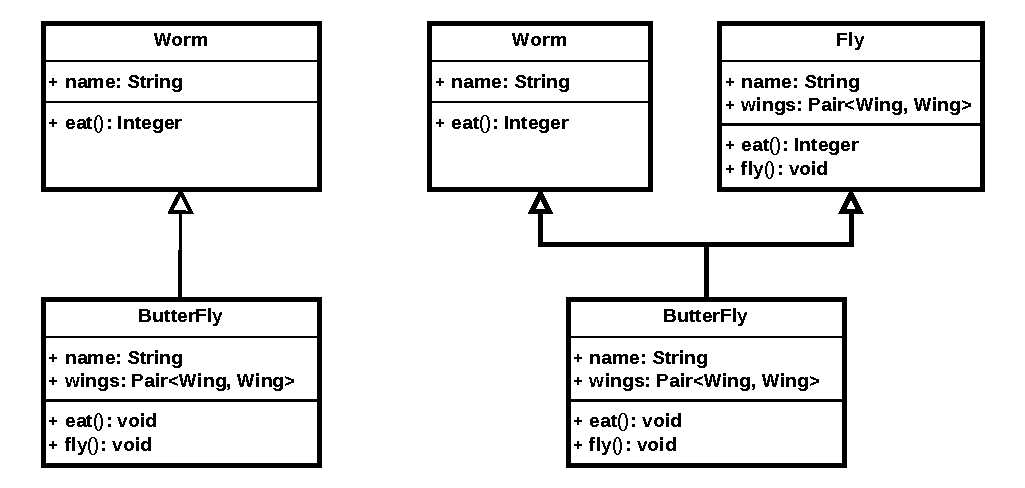
\includegraphics[width=0.9 \linewidth ]{pic/Inheritance-1.pdf}
	%\begin{block}{\textbf{Possible Problems}}
	\begin{itemize}
		\item \textbf{Conflict of method names} 
		\item \textbf{Repetition or duplication of information}
	\end{itemize}
	%\end{block}
\end{frame}
\begin{frame}[fragile]{\textbf{OOP: Multiple inheritance and} \texttt{Java}}
	A class can be derived from more than one superclass in \texttt{Python}. 
	\begin{lstlisting}[style=javaStyle]
class Worm:
	def __init__ (self, name): 
		self.name = name
	def eat(self): 
		print(self.name +" swallows")
class Fly:
	def __init__ (self, name): 
		self.name = name
	def eat(self): 
		print(self.name +" is nibbling..")
class ButterFly(Worm, Fly): 
	pass\end{lstlisting}
	\textbf{In Java}: How can we implement it? (Home work (1))
\end{frame}


\begin{frame}[fragile]{\textbf{OOP: Composition (has-a, delegation)}}
	Composition is an OOP concept that models the relationship \textbf{has-a}. 
	\begin{itemize}
		\item \textbf{Composite class}: \textbf{has a} components and \textbf{delegates} work to them.
		\item \textbf{Component class}: part of the composite class
	\end{itemize}
	
	\textbf{Example}: We already used it in the previous Example, but how and where? (Home work (2))
	
	\begin{block}{Remarks}
		\begin{itemize}
			\item More \textbf{flexible} compared to inheritance
			\item Changes to the component class have minimal or no effects on the composite class
			\item Better \textbf{encapsulation}, but a bit more wiring.
		\end{itemize}
	\end{block}
\end{frame}

\begin{frame}[fragile]{Example of Composition in \texttt{Java}}
	\begin{lstlisting}[style=javaStyle]
public class Fly {
	public String name; 
	public Pair<Wing, Wing> wings;
	
	public Fly(String name, Wing left, Wing right) {
		this.name = name;
		this.wings = Pair.with(left, right);
	}
	
	public void eat() {
		System.out.println(this.name +" is nibbling...");
	}
	public void fly() {
		System.out.println("Hi! I believe I can fly. ");
	}}\end{lstlisting}
\end{frame}

\begin{frame}[fragile]{\textbf{Example of Composition in} \texttt{Java}}
	\begin{lstlisting}[style=javaStyle]
public class Wing {
	public String name = null; 
	public Integer length = 4;
	public String wingColor = "white"; 
	
	public Wing() {}
	
	public Wing(String name, Integer length, String color) {
		this.name = name ; 
		this.length = length; 
		this.wingColor = color;
	}
}\end{lstlisting}
\end{frame}



\section{\textbf{Takeaway}}
\begin{frame}[fragile]{\textbf{Composition vs Inheritance (when to choose which)}}
	\begin{columns}[T,onlytextwidth]
		\column{0.50\textwidth}
		\textbf{Inheritance (is-a)}
		\begin{itemize}
			\item \textit{Pros}: Simple reuse, polymorphism via base type.
			\item \textit{Cons}: Tight coupling to base; fragile base class; LSP risks.
			\item \textit{Use when}: True subtype, stable base API, shared behaviour.
		\end{itemize}
		\column{0.50\textwidth}
		\textbf{Composition (has-a)}
		\begin{itemize}
			\item \textit{Pros}: Replaceable parts, multiple change axes, better encapsulation.
			\item \textit{Cons}: More wiring; no automatic access to base internals.
			\item \textit{Use when}: Need variability, combine features, avoid deep trees.
		\end{itemize}
	\end{columns}
	\vspace{0.9em}
	\textbf{Remarks:} Prefer composition for flexibility; use inheritance for true subtyping with stable behaviour.
\end{frame}

\section{\textbf{Home Work 1.0}}
\begin{frame}{\textbf{Questions}}
	\begin{enumerate}
		\item Consider the Multiple inheritance UML class diagram on \textbf{Slide 18}:
		\begin{enumerate}
			\item [a. ] Use the nation of Interface to implement that diagram
			\item[b. ] How can we solve the conflict of method names in \texttt{Python}?
		\end{enumerate}
		\item Given the \texttt{Java} Class Rectangle in \textbf{Slide 11}: 
		\begin{enumerate}
			\item[a. ] Find where the composition is being used
			\item[b. ] Can we replace that by an Inheritance relationship? 
			\item [c. ] How can this example illustrate the polymorphism?
		\end{enumerate}
		\item When would \textbf{inheritence} still be the cleaner choice?
	\end{enumerate}
	
	%\vspace{0.5cm}
	%\noindent\textbf{Solution to Challenge:} For 4KB pages, frame 21 starts at \texttt{21*4096 = 0x21000}; add offset 0x004: \texttt{0x21004}.
	
\end{frame}

\section{\textbf{What Next?}}

\begin{frame}{\textbf{What next?}}
	\begin{block}{}
		\vspace{0.1cm}
		Encapsulation, Polymorphism, and other Class relationships, e.g., association, aggregation, etc...
	\end{block}
\end{frame}
\begin{frame}{\textbf{Beyond OOP}}
	\begin{enumerate}
		\item Domain Driven Design (DDD)
		\item Agent Oriented Programming (AOP)
		\item Design Paterns
	\end{enumerate}
	\begin{block}{\textbf{Some Important Materials}}
		\begin{itemize}
			\item  Bloch, Joshua. Effective Java. 3rd ed. Addison-Wesley, 2018. 
			\item Gamma, Erich; Helm, Richard; Johnson, Ralph; Vlissides, John. Design Patterns: Elements of Reusable Object-Oriented Software. Addison-Wesley, 1994. 
			
			\item \href{https://github.com/lemerleau/OOP-JAVA.git}{Code and Course Material}
		\end{itemize}
	\end{block}
\end{frame}


\end{document}
